\documentclass[10pt]{beamer}

% ------------------------------------------------------------------------
% Carga de tu preámbulo personalizado (preamble.tex).
% Recuerda ponerlo en la misma carpeta para que \input funcione.
% ------------------------------------------------------------------------
\usetheme[progressbar=frametitle]{metropolis}
\usepackage{appendixnumberbeamer}
\usepackage{fancyvrb}
\usepackage{booktabs}
\usepackage[scale=2]{ccicons}
\usepackage{pgfplots}
\usepgfplotslibrary{dateplot}
\usepackage{type1cm}
\usepackage{lettrine}
\usepackage{ragged2e}
\usepackage{xspace}
\newcommand{\themename}{\textbf{\textsc{metropolis}}\xspace}
\usepackage{graphicx} % Allows including images
\usepackage{booktabs} % Allows the use of \toprule, \midrule and \bottomrule in tables
\usepackage[utf8]{inputenc} %solucion del problema de los acentos.
\usepackage{xcolor}
\definecolor{LightGray}{gray}{0.9}

\usepackage{minted}
\usemintedstyle{tango}
\newcommand{\mypyfile}[1]{\inputminted[linenos=true, fontsize=\footnotesize, frame=lines, framesep=5\fboxrule,framerule=1pt]{python}{#1}}

\setminted[python]{breaklines,frame=lines,framesep=2mm,baselinestretch=1.2,bgcolor=LightGray,linenos, fontsize=\footnotesize} % obeytabs=true, tabsize=2, showtabs=true}

%%%%%%%%%%%%%%%%%%%%%%%%%%%%%%%%%%%%%%%%%%%%%%%%%%%%%%%%%%%%%%%%%%%%%%%%%%%%%%%%%%%%%%
\setbeamercolor{progress bar}{fg=blue!50!black,bg=white!50!black}
\setbeamercolor{title separator}{fg=red!50!black,bg=white!50!black}
\setbeamercolor{frametitle}{fg=white!80!black,bg=red!50!black}
\title[PCFI161]{Programaci\'on para F\'isica y Astronom\'ia}
\subtitle{Departamento de Física.}

\newcommand{\myfront}{
\author[PCFI161]{Corodinadora: C Loyola \\ Profesoras/es C Loyola / C Femenías / Y Navarrete / C Ruiz}
\institute[UNAB]{Universidad Andrés Bello}
\date{Primer Semestre 2025}
}

\titlegraphic{%
  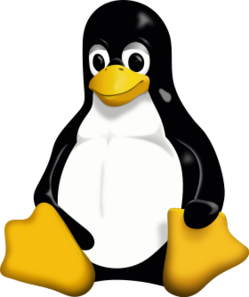
\includegraphics[width=.08\textwidth]{logo-tux.png}\hfill
  
\includegraphics[width=.3\textwidth]{logo-unab.png}\hfill
  
\includegraphics[width=.08\textwidth]{logo-python.png}
}

\makeatletter
\setbeamertemplate{title page}{
  \begin{minipage}[b][\paperheight]{\textwidth}
    \vfill%
    \ifx\inserttitle\@empty\else\usebeamertemplate*{title}\fi
    \ifx\insertsubtitle\@empty\else\usebeamertemplate*{subtitle}\fi
    \usebeamertemplate*{title separator}
    \ifx\beamer@shortauthor\@empty\else\usebeamertemplate*{author}\fi
    \ifx\insertdate\@empty\else\usebeamertemplate*{date}\fi
    \ifx\insertinstitute\@empty\else\usebeamertemplate*{institute}\fi
    \vfill
    \ifx\inserttitlegraphic\@empty\else\inserttitlegraphic\fi
    \vspace*{1cm}
  \end{minipage}
}
\makeatother


\makeatletter
\setlength{\metropolis@titleseparator@linewidth}{2pt}
\setlength{\metropolis@progressonsectionpage@linewidth}{2pt}
\setlength{\metropolis@progressinheadfoot@linewidth}{2pt}
\makeatother


\begin{document}

% ------------------------------------------------------------------------
% Portada de la Presentación
% ------------------------------------------------------------------------
\myfront{}

% ------------------------------------------------------------------------
% Slide 1: Título de la Sesión
% ------------------------------------------------------------------------
\begin{frame}
  \titlepage
  % Ejemplo:
  % \title{Semana 7 - Sesión 2 (Sesión 14): Aplicaciones Prácticas y Evaluación Parcial en Clase}
\end{frame}

% ------------------------------------------------------------------------
% Slide 2: Índice / Tabla de Contenidos
% ------------------------------------------------------------------------
\begin{frame}
  \frametitle{Resumen - Semana 7, Sesión 2 (Sesión 14)}
  \tableofcontents
\end{frame}

% ------------------------------------------------------------------------
% Configuración de bloques
% ------------------------------------------------------------------------
\metroset{block=fill}

% ----------------------------------------------------------------------------------------
% SECCIÓN 1: Introducción y Repaso
% ----------------------------------------------------------------------------------------
\section{Introducción y Repaso}

% ------------------------------------------------------------------------
% Slide 3: Conexión con la Semana 6 y la Sesión 7.1
% ------------------------------------------------------------------------
\begin{frame}{Repaso y Contexto}
  \begin{itemize}
    \item \textbf{Semana 6} nos introdujimos en:
      \begin{itemize}
        \item NumPy avanzado (\texttt{reshape}, \texttt{transpose}, \texttt{np.linalg}, etc.).
        \item Primeras visualizaciones con Matplotlib (gráficos 2D y un vistazo a 3D).
      \end{itemize}
    \item \textbf{Semana 7, Sesión 1 (Sesión 13)} cubrimos:
      \begin{itemize}
        \item Gráficas más avanzadas (subplots múltiples, histogramas, 3D).
        \item Breve introducción a \texttt{pandas} para manejar datos tabulares.
      \end{itemize}
    \item \textbf{Objetivo de hoy}: Resolver un problema evaluado (\textbf{Problema a Evaluar}), reforzar lo aprendido y seguir practicando la visualización y manejo de arreglos.
  \end{itemize}
\end{frame}

% ------------------------------------------------------------------------
% Slide 4: Objetivos de la Sesión 14
% ------------------------------------------------------------------------
\begin{frame}{Objetivos de la Sesión 14}
  \begin{itemize}
    \item \textbf{Aplicar} los conceptos de \textbf{NumPy} (manipulación avanzada, aleatoriedad, álgebra lineal) y \textbf{Matplotlib} (gráficas) en un ejercicio integrador.
    \item \textbf{Realizar} una \textbf{evaluación parcial} en grupos, donde se resolverá un problema práctico y se subirá a \textbf{CANVAS}.
    \item \textbf{Discutir} resultados y dificultades tras la entrega.
  \end{itemize}
\end{frame}

% ----------------------------------------------------------------------------------------
% SECCIÓN 2: Problema a Evaluar
% ----------------------------------------------------------------------------------------
\section{Problema a Evaluar (Evaluación en Clase)}

% ------------------------------------------------------------------------
% Slide 5: Descripción del Problema
% ------------------------------------------------------------------------
\begin{frame}{Problema a Evaluar: Análisis de Matriz Aleatoria y Visualización}
  \textbf{Contexto}:
  \begin{itemize}
    \item Queremos unir lo visto de \textbf{NumPy} avanzado y la \textbf{visualización} con Matplotlib.
    \item El objetivo es generar, manipular y analizar una \textbf{matriz aleatoria}, y luego presentar resultados en un \textbf{gráfico}.
  \end{itemize}
  
  \textbf{Tareas}:
  \begin{enumerate}
    \item Crear una \textbf{matriz} \(M\) de \textbf{tamaño 5x5} con valores enteros aleatorios en \([1, 10)\).
    \item Calcular \(\det(M)\), \(\text{traza}(M)\) y la \textbf{norma} Euclidiana de \(M\) (usar \(\texttt{np.linalg.norm}\)).
    \item Crear y graficar en 3D la \textbf{superficie} \(Z = f(X,Y)\) dada por:
    \[
      f(x,y) = \sin\left(\sqrt{x^2 + y^2}\right)
    \]
    con \(\texttt{x}\) e \(\texttt{y}\) en \([-5,5]\).
    \item \textbf{Incluir} en la misma figura (u otra subplot) un \textbf{histograma} de los valores de la matriz \(M\) (flattened).
  \end{enumerate}
\end{frame}

% ------------------------------------------------------------------------
% Slide 6: Instrucciones y Formato de Entrega
% ------------------------------------------------------------------------
\begin{frame}{Instrucciones para la Evaluación}
  \begin{itemize}
    \item Trabajar en \textbf{equipos de 2-3 estudiantes}.
    \item Abrir o crear un \textbf{notebook en Colab} (o un script local, si lo prefieren), llamarlo \texttt{Eval\_Semana7\_Apellidos.ipynb}.
    \item \textbf{Desarrollar} paso a paso el problema:
      \begin{enumerate}
        \item Generar y manipular la matriz \(M\).
        \item Calcular \(\det(M)\), traza y norma.
        \item Generar la \textbf{malla} (meshgrid) para la superficie 3D de \(\sin(\sqrt{x^2 + y^2})\).
        \item Graficar la superficie 3D \textbf{y} el \textbf{histograma} de valores en \(M\).
      \end{enumerate}
    \item Al finalizar (máximo \textbf{25-30 minutos}), \textbf{subir el archivo} a \textbf{CANVAS} (una entrega por grupo).
  \end{itemize}
\end{frame}

% ------------------------------------------------------------------------
% Slide 7: Pautas de Evaluación
% ------------------------------------------------------------------------
\begin{frame}{Pautas de Evaluación}
  \textbf{Se considerarán los siguientes criterios}:
  \begin{itemize}
    \item \textbf{Funcionalidad} (40\%): el código corre sin errores y cumple cada parte del problema.
    \item \textbf{Uso apropiado de NumPy} (20\%): buena manipulación de arreglos, \(\texttt{np.linalg}\), etc.
    \item \textbf{Visualización} (20\%): la gráfica 3D y el histograma están correctos y etiquetados (\texttt{title}, \texttt{xlabel}, \texttt{ylabel}, etc.).
    \item \textbf{Organización/Comentarios} (20\%): claridad del notebook o script, comentarios esenciales, legibilidad.
  \end{itemize}
  \vspace{0.3cm}
  \textbf{Nota}: Pueden agregar detalles extra (colormaps, formateo de texto, etc.) para mejorar la presentación.
\end{frame}

% ------------------------------------------------------------------------
% Slide 8: Tiempo de Desarrollo (25-30 min)
% ------------------------------------------------------------------------
\begin{frame}{Tiempo de Desarrollo}
  \begin{block}{}
    \huge{\textbf{Tienen 25-30 minutos para resolver y subir la solución a CANVAS.}}
  \end{block}
  \vspace{0.3cm}
  \textbf{Sugerencias}:
  \begin{itemize}
    \item Dividirse las tareas: uno genera la matriz y hace cálculos, otro arma la visualización.
    \item Revisar \texttt{plt.subplots} para combinar la vista 3D y el histograma.
    \item Testear con una semilla fija (\texttt{np.random.seed(...)}) si necesitan reproducibilidad.
  \end{itemize}
\end{frame}

% ----------------------------------------------------------------------------------------
% SECCIÓN 3: Trabajo y Discusión Posterior
% ----------------------------------------------------------------------------------------
\section{Trabajo y Discusión}

% ------------------------------------------------------------------------
% Slide 9: Espacio de Resolución y Entrega
% ------------------------------------------------------------------------
\begin{frame}{Espacio de Resolución}
  \begin{itemize}
    \item \textbf{En silencio o con discusión moderada}, cada grupo trabaja en su notebook.
    \item Cualquier duda puntual, pueden consultarme de forma breve sin interrumpir a otros grupos.
    \item Asegúrense de probar la ejecución completa antes de subir a CANVAS.
  \end{itemize}
\end{frame}

% ------------------------------------------------------------------------
% Slide 10: Cierre de la Evaluación
% ------------------------------------------------------------------------
\begin{frame}{Entrega Final}
  \begin{block}{Subida a CANVAS}
    \begin{itemize}
      \item Un integrante del grupo debe subir el \textbf{notebook .ipynb} (o .py) dentro del plazo acordado (25-30 min).
      \item Verifiquen que el archivo contenga todo el \textbf{código} y \textbf{gráficas} necesarias.
      \item \textbf{Comentarios básicos} o Markdown cells describiendo cada parte del problema.
    \end{itemize}
  \end{block}
  \vspace{0.3cm}
  \textbf{Tras la entrega}, discutiremos brevemente \textbf{soluciones} y \textbf{dificultades} encontradas.
\end{frame}

% ------------------------------------------------------------------------
% Slide 11: Discusión de Resultados
% ------------------------------------------------------------------------
\begin{frame}{Discusión Posterior}
  \begin{itemize}
    \item ¿Cómo resultó la experiencia de combinar \(\det\), \(\text{traza}\) y \(\text{norma}\) en la misma matriz?
    \item ¿Qué problemas técnicos surgieron con el \textbf{gráfico 3D}? (opciones de ejes, color map, etc.)
    \item ¿Fue sencillo combinar una gráfica 3D con un \textbf{histograma} en la misma figura (subplots)?
    \item ¿Opiniones sobre el tiempo asignado (25-30 min)? ¿Suficiente?
  \end{itemize}
\end{frame}

% ------------------------------------------------------------------------
% Slide 12: Resumen de la Evaluación
% ------------------------------------------------------------------------
\begin{frame}{Resumen de la Evaluación}
  \begin{itemize}
    \item La actividad integró:
      \begin{itemize}
        \item \textbf{Generación y manipulación} de una matriz aleatoria (Semana 6).
        \item \textbf{Cálculos algebraicos} (\texttt{np.linalg}).
        \item Visualización \textbf{3D} y un \textbf{histograma} en Matplotlib (Semana 6-7).
      \end{itemize}
    \item Apunta a \textbf{desarrollar fluidez} en la creación de figuras combinadas y análisis numérico.
    \item Revisión detallada de cada entrega se hará posterior a la clase, con retroalimentación.
  \end{itemize}
\end{frame}

% ----------------------------------------------------------------------------------------
% SECCIÓN 4: Cierre de la Sesión y Próximos Temas
% ----------------------------------------------------------------------------------------
\section{Cierre y Próximos Pasos}

% ------------------------------------------------------------------------
% Slide 13: Conclusiones de la Sesión 14
% ------------------------------------------------------------------------
\begin{frame}{Conclusiones de la Sesión 14}
  \begin{itemize}
    \item Se realizó un \textbf{ejercicio evaluado} integrando NumPy y Matplotlib.
    \item Reforzamos \textbf{conceptos de la semana 6} (álgebra lineal, manipulación de arreglos, gráficas).
    \item Discutimos \textbf{resolución} y \textbf{dificultades} en la práctica.
    \item Seguiremos ampliando la \textbf{visualización} y el \textbf{manejo de datos} en las próximas semanas.
  \end{itemize}
\end{frame}

% ------------------------------------------------------------------------
% Slide 14: Próxima Sesión
% ------------------------------------------------------------------------
\begin{frame}{Próximos Temas}
  \begin{itemize}
    \item \textbf{Semana 8}: Empezaremos \textbf{Unidad IV} (o V, según syllabus), enfocándonos en:
      \begin{itemize}
        \item Programación orientada a objetos (si corresponde).
        \item O profundizar en manejo de datos (pandas, estadística básica).
        \item Más ejemplos de visualización avanzada (scatter 3D, contour, animaciones).
      \end{itemize}
    \item \textbf{Retroalimentación individual} de esta evaluación se publicará en CANVAS.
  \end{itemize}
\end{frame}

% ------------------------------------------------------------------------
% Slide 15: Recursos Adicionales
% ------------------------------------------------------------------------
\begin{frame}{Recursos Adicionales}
  \begin{itemize}
    \item \href{https://numpy.org/doc/}{\textbf{NumPy Docs}} - Sección \texttt{numpy.linalg}.
    \item \href{https://matplotlib.org/3.1.1/gallery/index.html}{\textbf{Matplotlib Gallery}} - Ejemplos de todo tipo de gráficas (2D, 3D).
    \item \href{https://canvas.instructure.com/}{\textbf{CANVAS}} - Sección de entregas y feedback.
  \end{itemize}
\end{frame}

% ------------------------------------------------------------------------
% Slide 16: Cierre de la Sesión
% ------------------------------------------------------------------------
\begin{frame}
  \Huge{\centerline{¡Excelente trabajo y hasta la próxima!}}
  \vspace{0.5cm}
  \normalsize
  \begin{itemize}
    \item Recuerden revisar \textbf{notas y comentarios} en CANVAS.
    \item Continúen practicando la combinación NumPy + Matplotlib.
    \item ¡Nos vemos en la \textbf{Semana 8} con nuevos temas!
  \end{itemize}
\end{frame}

\end{document}

